\documentclass[11pt,a4paper]{article}

% --- Packages ---
\usepackage[utf8]{inputenc} 
\usepackage[T1]{fontenc}    
\usepackage{geometry}       
\geometry{
    a4paper,
    total={170mm,257mm},
    left=25mm,
    top=25mm,
}
\usepackage{graphicx}       
\usepackage{amsmath, amssymb} 
\usepackage{hyperref}       
\hypersetup{                
    colorlinks=true,
    linkcolor=blue,
    urlcolor=cyan,
}
\usepackage{indentfirst}
\usepackage{float}
\usepackage{listings}
\usepackage{xcolor}
\usepackage{tikz}
\usetikzlibrary{arrows.meta, positioning, shapes.geometric}

\lstset{
    basicstyle=\ttfamily\footnotesize,
    commentstyle=\color{green!60!black},
    keywordstyle=\color{blue},
    numbers=left,
    numberstyle=\tiny\color{gray},
    frame=single,
}

% Title and labeling
\title{Frequency Analysis \\ [1ex] \large ECSE 313 Group 16 Lab 3 Report}
\author{Nathaniel Hahn and Donovan Crowley}
\date{\today}

% Body
\begin{document}

\maketitle 

\tableofcontents 
\newpage

\section{Background}

\subsection{Synthesis of Periodic Signals}
Using the Fourier series expansion in the form

\begin{equation}
    s(t) = a_0 + \sum_{k=1}^{\infty} A_k sin(2\pi kf_0t + \theta_{k})
\end{equation}

for the two equations

\begin{equation}
    s_1(t) = rect(t - \frac{1}{2})
\end{equation}

\begin{equation}
    s_2(t) = rect(2t) - \frac{1}{2}
\end{equation}

The piecewise function in Equation 2 is only 1 from $t=0$ to $t=1$ and 0 elsewhere. Therefore, the function becomes:

\begin{equation}
    f_1(t) = \begin{cases}
                1\text{,} &  0 < t < 1 \\
                0\text{,} & 1 < t < 2
            \end{cases}
\end{equation}

Using a period ($T_0 = 2$) from $t \in [0, 2]$ and $f_0 = \frac{1}{T} = \frac{1}{2}$, the $a_0$ value of Equation 2 becomes

\begin{equation}
    a_0 = \frac{1}{T} \int_{0}^{T} f_1(t)dt = \frac{1}{2} \int_{0}^{1} 1dt = \frac{1}{2}
\end{equation}

The fundamental frequency of the function is $w_0 = \frac{2\pi}{T} = \pi$. Moreover, $a_k$ is

\begin{equation}
    a_k = \frac{2}{T} \int_{0}^{T} f_1(t)cos(kw_0t)dt = \int_{0}^{1} cos(k\pi t)dt = \frac{sin(k \pi)}{k\pi} = 0
\end{equation}

$a_k$ is zero because the sine function is zero for every integer value of k. The odd part of the signal, $b_k$, is defined as

\begin{equation}
    b_k = \frac{2}{T} \int_{0}^{T} f_1(t)sin(kw_0t)dt = \int_{0}^{1} sin(k\pi t)dt = \frac{1 - cos(k\pi)}{k\pi} 
\end{equation}

In Equation 7, when k is even, $b_k = \frac{1 - 1}{k\pi} = 0$. When k is odd, $b_k = \frac{1 - (-1)}{k\pi} = \frac{2}{k\pi}$.
Moreover, $A_k = b_k$ and $\theta_k = 0$. Thus, Equation 2 becomes

\begin{equation}
    s_1(t) = \frac{1}{2} + \sum_{k = 1, 3, 5, \dots}^{\infty} \frac{2}{k\pi} sin(\pi kt)
\end{equation}

\begin{figure}[h!]
    \centering
    
\includegraphics[width=0.75\linewidth]{image1.png}
    \caption{Sketch of Equation 2 from $[0, T_0]$}
\end{figure}



The piecewise function in Equation 3 is only $1-\frac{1}{2} = \frac{1}{2}$ from $t=-\frac{1}{4}$ to $t=\frac{1}{4}$ and $-\frac{1}{2}$ elsewhere. Therefore, the function becomes:

\begin{equation}
    f_2(t) = \begin{cases}
                \frac{1}{2}\text{,} & \lvert t \rvert < \frac{1}{4} \\
                -\frac{1}{2}\text{,} & \frac{1}{4} < \lvert t \rvert < \frac{1}{2}
            \end{cases}
\end{equation}

Since $f_2(t)$ is an even function (symmetric across the y-axis), $b_k = 0$.
Using a period ($T_0 = 1$) from $t \in [-\frac{1}{2}, \frac{1}{2}]$, the $a_0$ value of Equation 3 becomes

\begin{equation}
    a_0 = \frac{1}{T} \int_{-\frac{T}{2}}^{\frac{T}{2}} f_2(t)dt = \int_{-\frac{1}{2}}^{-\frac{1}{4}} -\frac{1}{2}dt + \int_{-\frac{1}{4}}^{\frac{1}{4}} \frac{1}{2}dt + \int_{\frac{1}{4}}^{\frac{1}{2}} -\frac{1}{2}dt = 0
\end{equation}

The fundamental frequency of the function is $w_0 = \frac{2\pi}{T} = 2\pi$ and $f_0 = \frac{1}{T} = 1$. Moreover, $a_k$ is

\begin{equation}
    a_k = \frac{2}{T} \int_{-\frac{T}{2}}^{\frac{T}{2}} f_2(t)cos(kw_0t)dt = 2\int_{-\frac{1}{2}}^{-\frac{1}{4}} -\frac{1}{2}cos(2\pi kt) + 2\int_{-\frac{1}{4}}^{\frac{1}{4}} \frac{1}{2}cos(2\pi kt) + 2\int_{\frac{1}{4}}^{\frac{1}{2}} -\frac{1}{2}cos(2\pi kt)
\end{equation}

\begin{equation}
    a_k = -\left[ \frac{sin(2\pi kt)}{2\pi k} \right]_{-\frac{1}{2}}^{-\frac{1}{4}} + \left[ \frac{sin(2\pi kt)}{2\pi k} \right]_{-\frac{1}{4}}^{\frac{1}{4}} - \left[ \frac{sin(2\pi kt)}{2\pi k} \right]_{\frac{1}{4}}^{\frac{1}{2}}
\end{equation}

\begin{equation}
    a_k = \frac{4sin(\frac{\pi k}{2}) - 2sin(\pi k)}{2\pi k} = \frac{2sin(\frac{k\pi}{2})}{k\pi}
\end{equation}

$A_k = a_k$. When $k$ is even, $A_k = 0$. For $k = 1, 5, \dots$, $A_k = \frac{2}{k\pi}$, and for $k = 3, 7, \dots$, $A_k = -\frac{2}{k\pi}$.
Additionally, converting the cosine function to sine function using the identity $cos(\theta) = sin(\theta + \pi/2)$, the $\theta$ values become $\theta = \frac{\pi}{2}$.
Since $A_k$ alternates by sign every other odd value, the $\theta$ value is positive for $k = 1, 5, \dots$ and negative for $k = 3, 7, \dots$.
Thus, Equation 3 becomes

\begin{equation}
    s_2(t) = \sum_{k = 1, 3, 5, \dots}^{\infty} \frac{2}{k\pi} sin(2\pi kt + \theta)
\end{equation}

where $\theta = \frac{\pi}{2}$ for $k = 1, 5, \dots$ and $\theta = - \frac{\pi}{2}$ for $k = 3, 7, \dots$

\begin{figure}[h!]
    \centering
    
\includegraphics[width=0.75\linewidth]{image2.png}
    \caption{Sketch of Equation 2 from $[-\frac{T_0}{2}, \frac{T_0}{2}]$}
\end{figure}

\subsection{Magnitude and Phase of Discrete-Time Systems}

For the following function:

\begin{equation}
    y(n) = 0.9y(n - 1) + 0.3x(n) + 0.24x(n - 1)
\end{equation}

By setting $x(n) = \delta(n)$, the impulse reponse is found through setting $n = 0$.

\begin{equation}
    y(0) = 0.9y(-1) + 0.3\delta(0) + 0.24\delta(-1) = 0.9(0) + 0.3(1) + 0.24(0) = 0.3
\end{equation}

\begin{equation}
    y(1) = 0.9y(0) + 0.3\delta(1) + 0.24\delta(0) = 0.9(0.3) + 0.3(0) + 0.24(1) = 0.51
\end{equation}

For $n > 1$, Equation 15 is just $y(n) = 0.9y(n-1)$. Therefore the impulse is

\begin{equation}
    h(n) = 0.3\delta(n) + 0.51(0.9)^{n-1} u(n-1)
\end{equation}

The system diagram of Equation 15 is shown in Figure 3.



\begin{figure}[h]
\centering
\resizebox{\textwidth}{!}{%
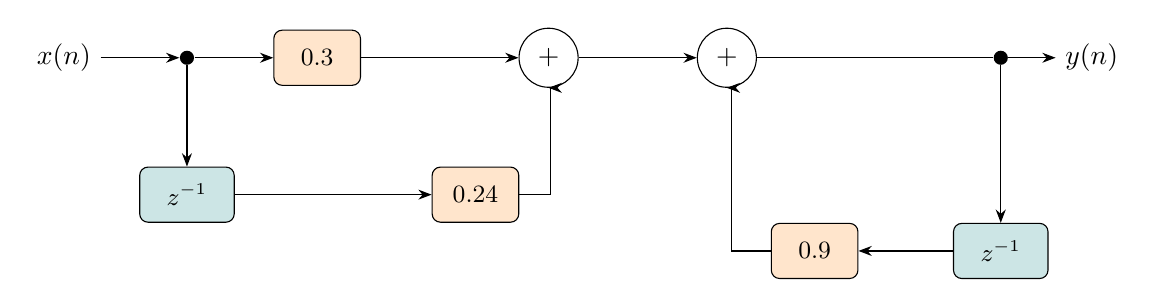
\begin{tikzpicture}[
    >=Stealth,
    node distance=1.6cm,
    block/.style={
        draw, rectangle, minimum width=1.2cm, minimum height=0.7cm,
        rounded corners=3pt, fill=teal!20, font=\small
    },
    gain/.style={
        draw, rectangle, minimum width=1.1cm, minimum height=0.7cm,
        rounded corners=3pt, fill=orange!20, font=\small
    },
    sum/.style={
        draw, circle, minimum size=0.75cm, font=\normalsize
    },
    dot/.style={
        circle, fill, inner sep=1.8pt
    }
]

\node (xn) {$x(n)$};

\node [dot, right=1.0cm of xn] (xbranch) {};

\node [gain, right=1.0cm of xbranch] (g03) {$0.3$};

\node [sum, right=2cm of g03] (sum1) {$+$};

\node [sum, right=1.5cm of sum1] (sum2) {$+$};

\node [dot,  right=3.0cm of sum2] (ybranch) {};
\node [right=0.6cm of ybranch]    (yn)      {$y(n)$};

\node [block, below=1.285cm of xbranch] (zff) {$z^{-1}$};

\node [gain,  right=2.5cm of zff] (g024) {$0.24$};

\node [block, below=2cm of ybranch] (zfb) {$z^{-1}$};

\node [gain,  left=1.2cm of zfb]  (g09) {$0.9$};

\draw[->] (xn) -- (xbranch);

\draw[->] (xbranch) -- (g03);

\draw[->] (g03) -- (sum1);

\draw[->] (sum1) -- (sum2);

\draw[-]  (sum2) -- (ybranch);
\draw[->] (ybranch) -- (yn);

\draw[->] (xbranch) -- ++(0,-1.285cm) -| (zff.north);
\draw[->] (zff) -- (g024);

\draw[->] (g024.east) -- ++(0.4,0) |- (sum1.south);

\draw[->] (ybranch) -- ++(0,-2.0cm) -- (zfb.north);

\draw[->] (zfb) -- (g09);

\draw[->] (g09.west) -- ++(-0.5,0) |- (sum2.south);

\end{tikzpicture}
}
\caption{Direct Form I: $y(n)=0.9\,y(n-1)+0.3\,x(n)+0.24\,x(n-1)$}
\label{fig:directform1}
\end{figure}

The Z-transform of Equation 15 is found using the equation $x(n-k) \leftrightarrow z^{-k}X(z)$

\begin{equation}
    Y(z) = 0.9z^{-1}Y(z) + 0.3X(z) + 0.24z^{-1}X(z)
\end{equation}

The transfer function of Equation 15 using Equation 19 is 

\begin{equation}
    (1 - 0.9 z^{-1})Y(z) = (0.3 + 0.24z^{-1})X(z)
\end{equation}

\begin{equation}
    H(z) = \frac{0.3 + 0.24z^{-1}}{1 - 0.9 z^{-1}}
\end{equation}

The magnitude and phase responses of Equation 21 are plotted in Figure 4

\begin{figure}[h!]
    \centering
    
\includegraphics[width=0.75\linewidth]{image3.png}
    \caption{Discrete-Time Magnitude and Phase Responses of Equation 21}
\end{figure}

\section{Continuous-Time Frequency Analysis}

\subsection{Synthesis of Periodic Signals}

\subsection{Modulation Property}

\subsection{System Analysis}

\section{Discrete-Time Frequency Analysis}

\subsection{Discrete-Time Fourier Transform}

\subsection{System Analysis}

\end{document}
